\renewcommand{\figurename}{Photo}
\renewcommand{\tablename}{Table}
\renewcommand{\labelitemii}{$\star$}

\newpage
\section{Arkadiusz Paterak: A bit of astronomy}
\label{sec:arekpaterak}

\subsection{Stefan–Boltzmann equation}
The Stefan–Boltzmann equation applied to a black body gives the value for luminosity for a black body, an idealized object which is perfectly opaque and non-reflecting: 

\[ L=\sigma AT^4 \]

The surface area of a sphere with radius r is \( A=4\pi r^2 \), so for stars and other point sources of light:

\[ L= 4\pi\sigma r^2T^4 \]

\subsection{Hubble Deep Field}
The Hubble Deep Field (see Photo \ref{fig:deepfield}) is an image of a small region in the constellation Ursa Major, constructed from a series of observations by \textbf{the Hubble Space Telescope}. 

\begin{figure}[H]
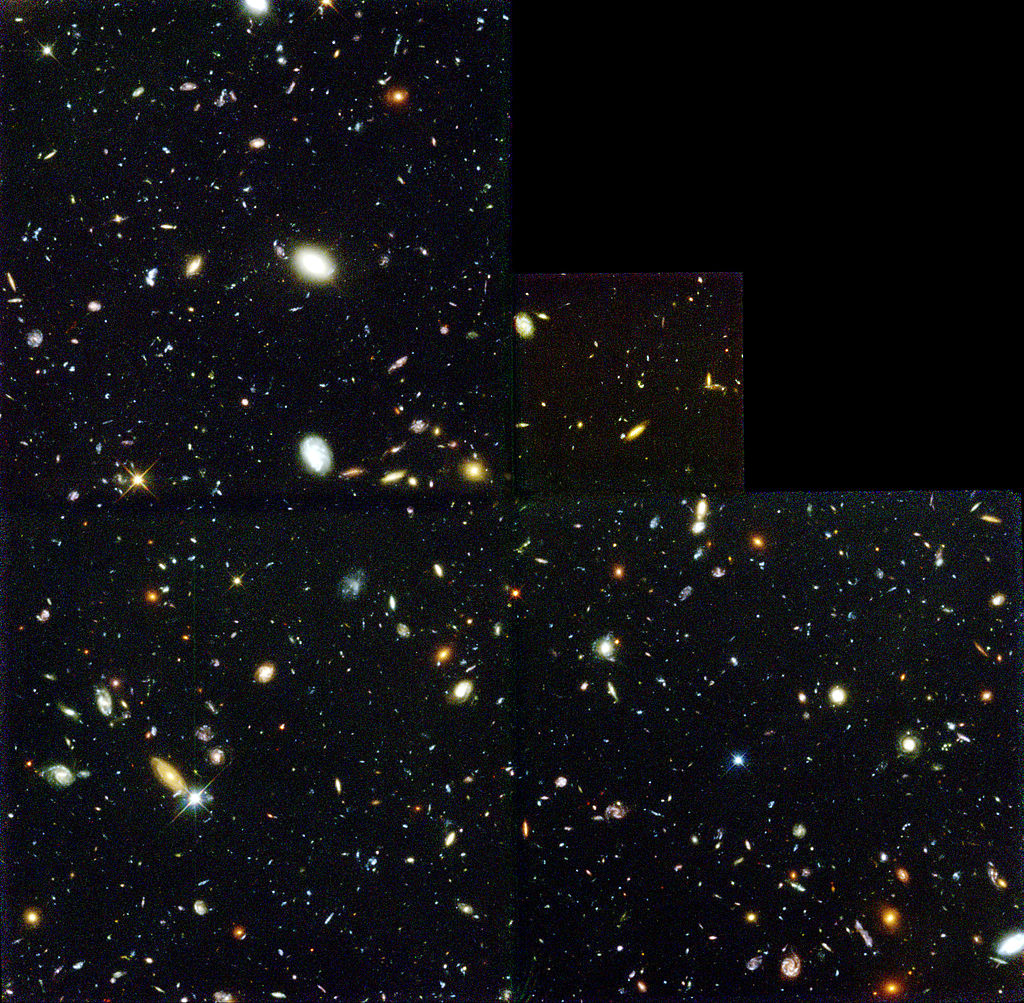
\includegraphics[scale=1]{arek/hdf}
\centering
\caption{Hubble Deep Field}
\label{fig:deepfield}
\end{figure}

The field is so small that only a few foreground stars in the Milky Way lie within it; thus, almost all of the 3,000 objects in the image are \underline{galaxies} . By revealing such large numbers of very young galaxies, the HDF has become \textbf{a landmark image in the study of the early universe}.


\subsection{Stellar classification}
One example of a classification of stars is Harvard spectral classification (see Table \ref{tab:starclass}).
\begin{table}[H]
\resizebox{\textwidth}{!}{\begin{tabular}{|c|m{2.5cm}|l|l|l|l|m{3cm}|}
\hline
Class & Effective temperature & Colour                               & Mass (\(M_\odot\))           & Radius (\(R_\odot\))           & Luminosity (\(L_\odot\))         & \% of all main-sequence stars \\ \hline
O     & $\geq$ 30000 K  & \cellcolor[HTML]{3166FF}blue         & $\geq$ 16 & $\geq$ 6.6 & $\geq$ 30000 & $\sim$0.00003\%               \\ \hline
B     & 10000 - 30000 K       & \cellcolor[HTML]{34CDF9}blue white   & 2.1 - 16        & 1.8 - 6.6        & 25 - 30000         & 0.13\%                        \\ \hline
A     & 7500 - 10000 K        & \cellcolor[HTML]{DAE8FC}white        & 1.4 - 2.1       & 1.4 - 1.8        & 5 - 25             & 0.6\%                         \\ \hline
F     & 6000 - 7500 K         & \cellcolor[HTML]{FFFFC7}yellow white & 1.04 - 1.4      & 1.15 - 1.4       & 1.5 - 25           & 3\%                           \\ \hline
G     & 5200 - 6000 K         & \cellcolor[HTML]{FFFE65}yellow       & 0.8 - 1.04      & 0.96 - 1.15      & 0.6 - 1.5          & 7.6\%                         \\ \hline
K     & 3700 - 5200 K         & \cellcolor[HTML]{FFCB2F}light orange & 0.45 - 0.8      & 0.7 - 0.96       & 0.08 - 0.6         & 12.1\%                        \\ \hline
M     & 2400 - 3700 K         & \cellcolor[HTML]{F56B00}orange red   & 0.06 - 0.45     & \textless 0.7    & \textless 0.08     & 76.45\%                       \\ \hline

\end{tabular}}
\caption{Harvard spectral classification}
\label{tab:starclass}
\end{table}

\subsection{Circumpolar stars}
A circumpolar star is a star, as viewed from a given latitude on Earth, that never sets below the horizon due to its apparent proximity to one of the celestial poles.

The northern circumpolar constellations for Poland:
\begin{itemize}[label=$\star$]
    \item Cepheus 
    \item Cassiopeia 
    \item Ursa Minor
    \item Draco
    \item Ursa Major
    \item Camelopardalis
\end{itemize}

\subsection{Planets of the Solar System}
\begin{enumerate}
    \item Mercury
    \item Venus
    \item Earth
    \item Mars
    \item Jupiter
    \item Saturn
    \item Uranus
    \item Neptune
\end{enumerate}